\documentclass{article}

\usepackage[dutch]{babel}
\usepackage{epsfig}
\usepackage{verbatim}
\usepackage{moreverb}
\usepackage{float}
\usepackage{graphicx}
\usepackage{framed}
\usepackage{chngcntr}
\usepackage{enumitem}
\usepackage{verbdef}
\usepackage{mathtools}
\usepackage{url} 
\usepackage[font=bf]{caption}
\usepackage{amsmath}

\author{Peter van Dijk \& Elizabeth Schermerhorn}
\date{\today}
\title{Lokalisatie met Arduino$`$s op basis van vier bakens}
\begin{document}
\maketitle
\newpage
\tableofcontents
\clearpage
\section{Inleiding}
Dit is het verslag voor de opdracht 'Lokalisatie' van het vak Networked Smart Systems. Voor deze opdracht moest er een lokalisatiealgoritme worden ontwikkeld waarmee binnen een vak van 5 bij 5 meter de positie zo nauwkeurig mogelijk proberen te bepalen. Hierbij wordt gebruik gemaakt van ultrasone signalen vanuit vaste referentiepunten op de hoeken van dit vak. De locatie van een meetinstrument kan van belang zijn bij het verrichtingen van metingen, bijvoorbeeld bij een branddetector in een bos. \\
\\
In dit paper zal het door ons ge\"{i}mplementeerde lokalisatiealgoritme besproken worden. Er zal eerst een afweging worden gemaakt tussen bestaande algoritmen. Daarna zal de gebruikte hardware en software voor de lokalisatie besproken worden. Vervolgens wordt er uit deze algoritmen het algoritme gekozen dat het beste aansluit op deze hardware en software en de implementatie hiervan uitgelegd worden. Daaropvolgend zullen de testopstelling en de resultaten worden uitgelicht. Ten slotte zal hieruit een conclusie worden getrokken en zullen er aanbevelingen voor vervolgonderzoek gedaan worden.


\section{Probleemstelling}
Aan de hand van vier bakens die in een 5 bij 5 meter veld geplaatst worden, moet de positie van de ontvanger bepaald worden. De onderzoeksvraag die hier centraal staat: \textit{"Is het mogelijk om met een afwijking kleiner dan 5 procent de positie van de ontvanger in een 5 bij 5 meter veld te bepalen?"}
De verwachte uitkomst van dit onderzoek is dat het eindproduct in staat is om met een nauwkeurigheid van 25 centimeter (5 procent) de positie te bepalen binnen het 5 bij 5 meter veld. \\
\\
Een limitatie bij deze positiebepaling is onder andere de gebruikte hardware. Er wordt gebruik gemaakt van een Arduino Uno, een computer met beperkte rekenkracht en beperkt werkgeheugen.\cite{uno}
Verwachte obstakels hierdoor zijn bit overflows en het beperkte aantal variabelen in de code (in verband met het beperkte werkgeheugen). De overflow wordt als probleem verwacht omdat de Arduino geen grote getallen kan representeren en er waarschijnlijk met grote getallen gerekend moet gaan worden. Een voorbeeld hiervan is bijvoorbeeld de halvering van het bereik van getallen. Zo is een \texttt{long} geen 64, maar 32 bits.\cite{long} Een ander verwacht obstakel is de snelheid van het geluidsignaal dat de bakens zullen gaan uitzenden, omdat de geluidssnelheid varieert naarmate de temperatuur en luchtvochtigheid veranderen. Dit zou gevolgen kunnen hebben voor de te bepalen positie.  


\section{Gerelateerd werk}
Op het gebied van lokalisatie-algoritmen is er al veel onderzoek verricht. Hierdoor is er veel werk wat gebruikt kan worden bij het onderzoek. Er zullen twee papers worden bekeken waarin globale positie systemen (GPS) beschreven worden. In de twee papers worden er trilateratie-algoritmen gepresenteerd waarmee de exacte locatie bepaald kan worden op twee verschillende manieren. In \textit{A New Location Technique for the Active Office} worden twee manieren beschreven \cite{ward97}, namelijk:
\begin{itemize}
	\item Active badges
	\item ParcTab
\end{itemize}
Active Badges is gebaseerd op het periodiek verzenden van informatie naar iedereen. Door bijvoorbeeld een gebouw heen zijn er overal sensoren geplaatst die luisteren naar berichten die worden verstuurd door badges. Door vast te stellen welke sensoren het signaal van welke badge hebben ontvangen is het mogelijk een grove schatting te geven van de locatie van de badge.\\
\\
ParcTab is een zakcomputer die gebruik maakt van een netwerk dat communiceert via infraroodsignalen. Wat betreft de lokalisatie lijkt deze heel veel op de badges die hiervoor zijn beschreven. Er worden berichten verstuurd en afhankelijk van welke sensor deze ontvangen wordt de locatie bepaald. Een groot verschil is dat de ParcTab is bedoeld voor intensiever gebruik dan alleen het berekenen van de locatie. \\
\\
In het algoritme in het hoofdstuk \textit{Localization and positioning} van \textit{Protocols and Architectures for Wireless Sensor Networks} wordt er gebruik gemaakt van bakens die een signaal uitzenden \cite{h9}. Met behulp van deze bakens kan op twee manieren een positie worden berekend: met \emph{triangulatie} (Figuur \ref{triangulatie}) en \emph{trilateratie} (Figuur \ref{trilateratie}). Triangulatie maakt gebruik van de invalshoek om de positie te berekenen. Hierbij moeten de hoeken tot tenminste twee bakens en de afstand tussen de bakens bekend zijn. Trilateratie gebruikt de afstand tot de bakens om de positie te bepalen. Voor dit algoritme is het van belang dat er minimaal tot drie bakens de afstand bekend is. Wanneer de afstand tot drie bakens bekend is kan met een simpele matrixvermenigvuldiging de positie berekend worden. Dit is het algoritme dat ook is gebruikt in de in dit paper besproken oplossing.
\begin{figure}[h]
\centering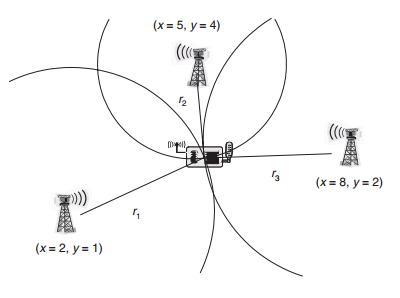
\includegraphics[scale=0.75]{trilateratie.png}
\caption{Trilateratie \cite{h9}}
\label{trilateratie}
\end{figure}
\begin{figure}[h]
\centering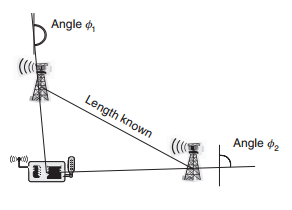
\includegraphics[scale=0.75]{triangulatie.png}
\caption{Triangulatie \cite{h9}}
\label{triangulatie}
\end{figure}\\
\\
De opstelling die hier gebruikt wordt zal als basisprincipe worden gebruikt voor de implementatie beschreven in deze paper. Aangezien in dit experiment ook gebruik wordt gemaakt van bakens die een signaal versturen en een ontvanger die dit ontvangt en op basis van die gegevens de positie bepaald. 

\section{Het algoritme}
Het algoritme dat ge\"{i}mplementeerd is bestaat uit twee verschillende onderdelen. Het eerste deel bestaat uit het berekenen van de afstand tot de bakens en het tweede deel uit de berekening van de positie. Deze twee onderdelen zullen apart besproken worden voor de overzichtelijkheid.
	
\begin{figure}[h]
\centering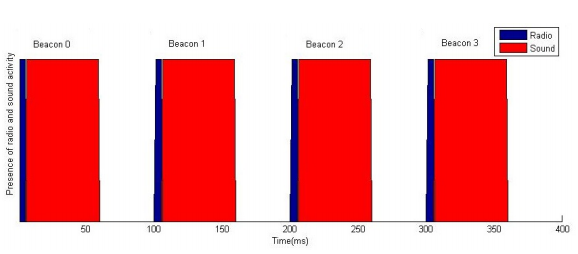
\includegraphics[]{berichten_bakens.png}
\caption{Het signaal van de bakens}
\label{uitzenden_bakens}
\end{figure}
	
\subsection{Afstand bepalen tot aan de bakens}
Zoals te zien is in Figuur \ref{uitzenden_bakens} wordt er eerst een radiosignaal verstuurd, gevolgd door een ultrasoon signaal. De bakens gebruiken een master-slave opstelling, waarbij de master aangeeft wanneer elke slave mag sturen. Als eerste wordt er door de master-baken een radio uitzending uitgevoerd met als bericht het ID van de baken die vervolgens mag zenden. Omdat dit een radiosignaal is gaat dit met de snelheid van het licht, hierdoor is het tijdsverschil tussen de verschillende nodes die het op verschillende momenten ontvangen verwaarloosbaar. Op het moment dat het radiosignaal ontvangen wordt, begint de desbetreffende baken direct met het zenden van een ultrasoon geluid. Er is bekend dat dit meteen gebeurt, dus door bij te houden hoeveel tijd verstrijkt tussen het ontvangen van het radiosignaal en het ontvangen van het ultrasoon geluid kan er een schatting gemaakt worden van de afstand tussen baken en ontvanger met behulp van de geluidssnelheid. De berekening hiervoor ziet er als volgt uit:\\
\\
	\indent$ d_b = (T_u- T_r) * g $\\
	\\
	Met:\\
	\\
	\indent$ d_b$: afstand tot baken\\
	\indent$T_u$: tijd ontvangen ultrasoon geluid\\
	\indent$T_r$: tijd ontvangen radio\\
	\indent$g$: geluidssnelheid\\
\\
De geluidssnelheid is afhankelijk van temperatuur en luchtvochtigheid. Het is van belang om een juiste (constante) waarde voor de geluidssnelheid te kiezen die rekening houdt met de omgeving waarin het systeem zich bevindt, om afwijkingen in de meetresultaten te minimaliseren. Het proces van luisteren en berekenen herhaalt zich oneindig lang zodat wanneer de node in beweging is er nog steeds een correcte locatie berekend kan worden. 
	
\subsection{Trilateratie}
Wanneer van alle vier de bakens bekend is wat hun afstand is tot de node, kan door middel van matrixberekeningen de positie worden bepaald. Hierbij is er gebruik gemaakt van het hoofdstuk \textit{Localization and positioning} van \textit{Protocols and Architectures for Wireless Sensor Networks}\cite{h9}. Alle afstanden en berekende uitkomsten worden weergegeven in centimeters om de nauwkeurigheid te kunnen bepalen. \\
De volgende berekening is gebruikt bij het berekenen van de locatie: \\
\\
\indent$2*\begin{bmatrix}
       x_3 - x_1 & y_3 - y_1 \\
       x_3 - x_2 & y_3 - y_2 \\          
                
     \end{bmatrix}
     \begin{bmatrix}
       x_u \\          
       y_u \\         
     \end{bmatrix}
=\begin{bmatrix}
       (r_1^2 - r_3^2) - (x_1^2 - x_3^2) - (y_1^2 - y_3^2) \\
       (r_2^2 - r_3^2) - (x_2^2 - x_3^2) - (y_2^2 - y_3^2) \\
     \end{bmatrix}$ \\
 \\
Met: \\
\\
\indent$x_u$: de te berekenen x-co\"{o}rdinaat van de Arduino.\\
\indent$y_u$: de te berekenen y-co\"{o}rdinaat van de Arduino.\\
\indent$x_i$: het x-co\"{o}rdinaat van baken $i$.\\
\indent$y_i$: het y-co\"{o}rdinaat van baken $i$.\\
\indent$r_i$: de afstand van de Arduino tot aan baken $i$.

\subsection{Implementatie}
De matrixvermenigvuldiging voor de trilateratie is om te schrijven naar de volgende formules, waarmee de x- en y-co\"ordinaten van de ontvanger te berekenen zijn: \\
\\
\indent$c_1 = (((r_1*r_1)-(r_3*r_3))-((x_1*x_1)-(x_3*x_3))-((y_1*y_1)-(y_3*y_3)))/2 $\\
\\
\indent$c_2 = (((r_2*r_2)-(r_3*r_3))-((x_2*x_2)-(x_3*x_3))-((y_2*y_2)-(y_3*y_3)))/2 $\\
\\
\indent$n =(-((y_3-y_1)*10000)/(x_3-x_1)) $\\
\\
\indent$m = ((c_1*10000)/(x_3-x_1)) $\\
\\
\indent$y_u = ((c_2*10000) - m*(x_3-x_2))/(n*(x_3-x_2) + (10000*(y_3-y_2))) $\\
\\
\indent$x_u = ((n*y)+m)/10000 $\\
\\
Wat opvalt aan deze berekening is dat er een aantal maal $10.000$ in staat. Deze factor is ge\"introduceerd om te voorkomen dat afkapping van getallen zorgt voor foute resultaten. Als deze factor niet gebruikt zou worden dan zouden tussenberekeningen een getal kleiner dan $1$ kunnen opleveren, wat afgekapt wordt tot $0$.  Hiermee doorrekenen levert incorrecte resultaten op. De factor wordt aan het einde weer weggedeeld, om het gewenste resultaat te verkrijgen. Een alternatief voor deze oplossing is het gebruik van decimale getallen, maar het rekenen hiermee is erg langzaam, daarom is daar niet voor gekozen.\\
\\
Doordat de afstand tot aan de bakens elke 400 milliseconden opnieuw wordt berekend geldt dit ook voor de x- en y-co\"{o}rdinaten. Voor elke vier nieuwe afstandsmetingen worden de x- en y-co\"ordinaten opnieuw berekend. Het algoritme maakt gebruik van alle vier de bakens en niet slechts drie voor de positiebepaling. Dit wordt gedaan als volgt. Voor elke combinatie van drie bakens wordt met behulp van de afstanden tot deze bakens met behulp van het hiervoor genoemde algoritme een set van co\"ordinaten berekend. Vervolgens wordt het gemiddelde genomen van de berekende sets co\"ordinaten. Dit zorgt er voor dat er voor kleine afwijkingen in afstandsberekening tot bakens gecompenseerd kan worden. In Appendix \ref{code} staat de code die de berekeningen implementeert.

\section{Testopstelling en metingen}
Om de implementatie te testen is er gebruik gemaakt van een testopstelling zoals die in Figuur \ref{Meetopstelling} staat weergegeven. In dit figuur staan de oranje co\"{o}rdinaten voor de bakens die het geluid uitzenden en de roze co\"{o}rdinaten staan voor de drie testposities die zijn gebruikt in dit experiment. Voor deze tests is er gebruik gemaakt van hardware en software waarbij de software bestaat uit een aantal gebruikte constanten. Eerst zal de hardware toegelicht worden, daarna de software en zal het testen samen met resultaten gegeven worden.  

\begin{figure}[h] 
\centering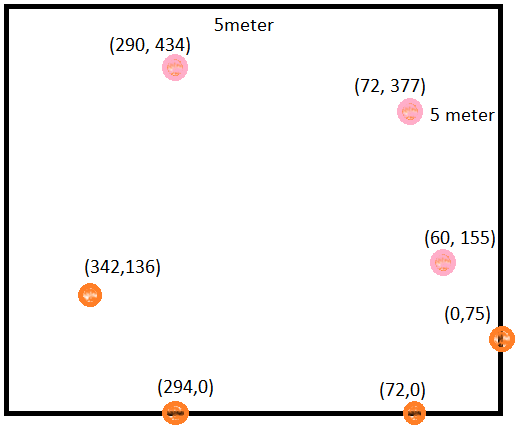
\includegraphics[scale=0.5]{Meetopstelling.png}
\caption{Meetopstelling}
\label{Meetopstelling}
\end{figure}

%De gebruikte hardware
\subsection{De hardware}
De hardware bestaat uit twee delen, er is een ontvanger die de geluidsgolven opvangt. Deze ontvanger bevindt zich op de Arduino. Er zijn tevens vier zenders, deze staan voor de vier bakens die worden gebruikt om het ultrasoongeluid uit te zenden. 
\subsubsection{Ontvanger}
De Hardware die gebruikt is voor het ontvangen van de signalen is een Arduino UNO en een Nordic nRF24L01 draadloze transceiver(kan ontvangen en zenden) in combinatie met een ultrasoonontvanger. In Figuur \ref{voorkant} en \ref{achterkant} staat de gebruikte ontvanger vanuit twee posities bekeken.
\begin{figure}[h]
\centering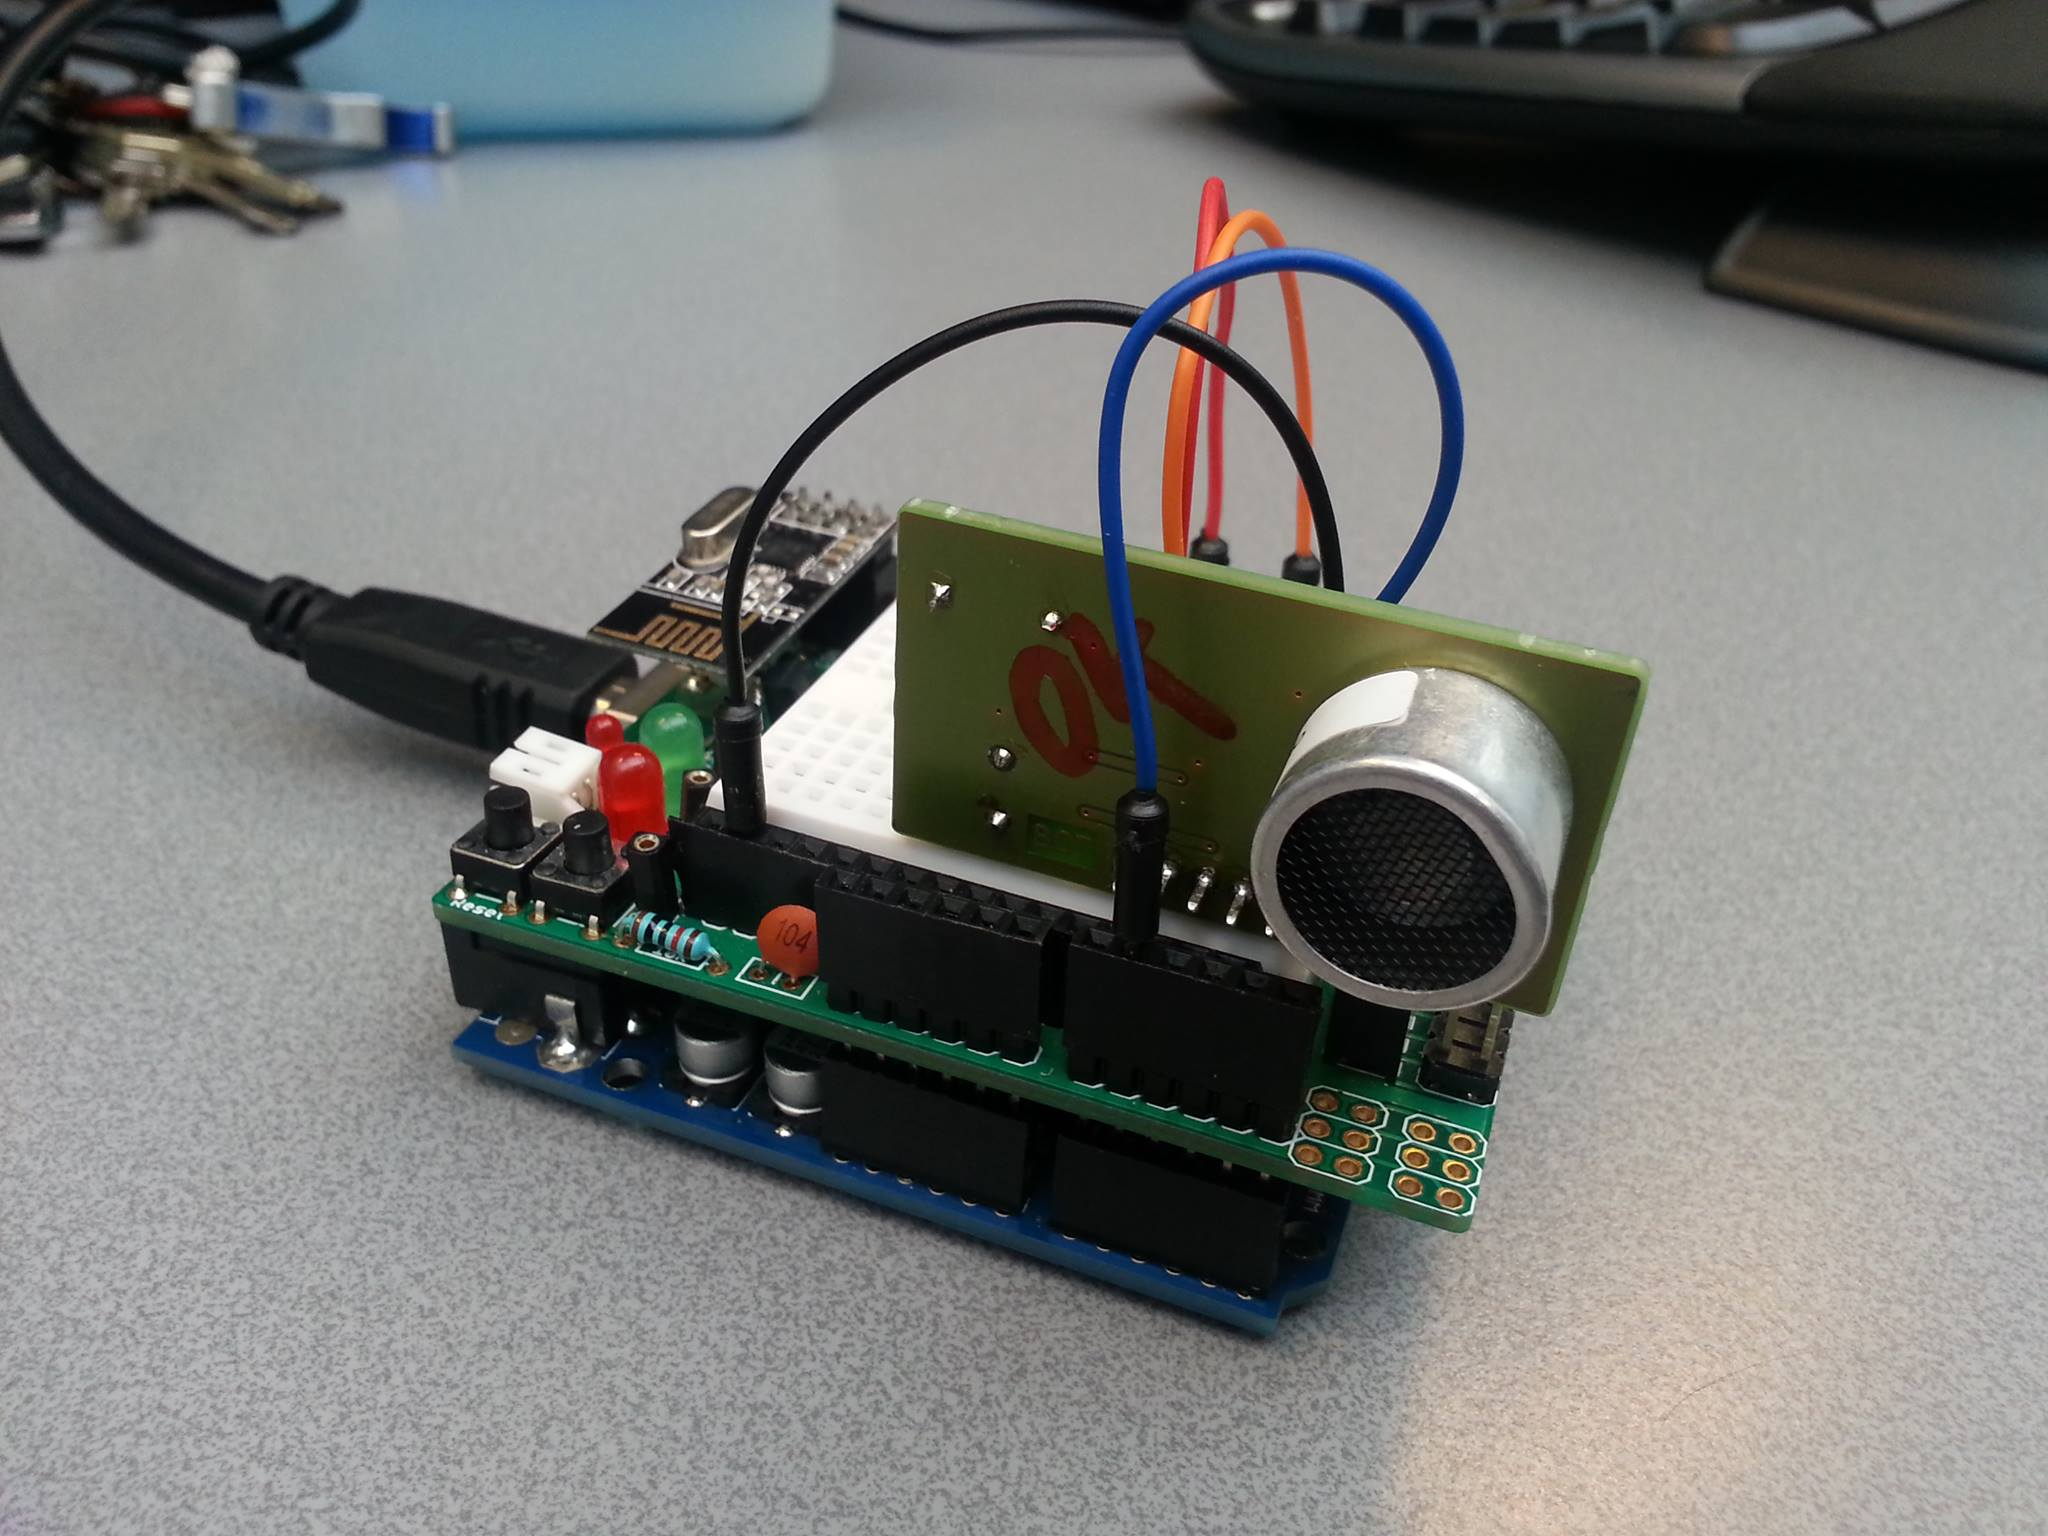
\includegraphics[scale=0.06]{voorkant.jpg}
\caption{De ontvanger (voorkant)}
\label{voorkant}
\end{figure}
\begin{figure}[h]
\centering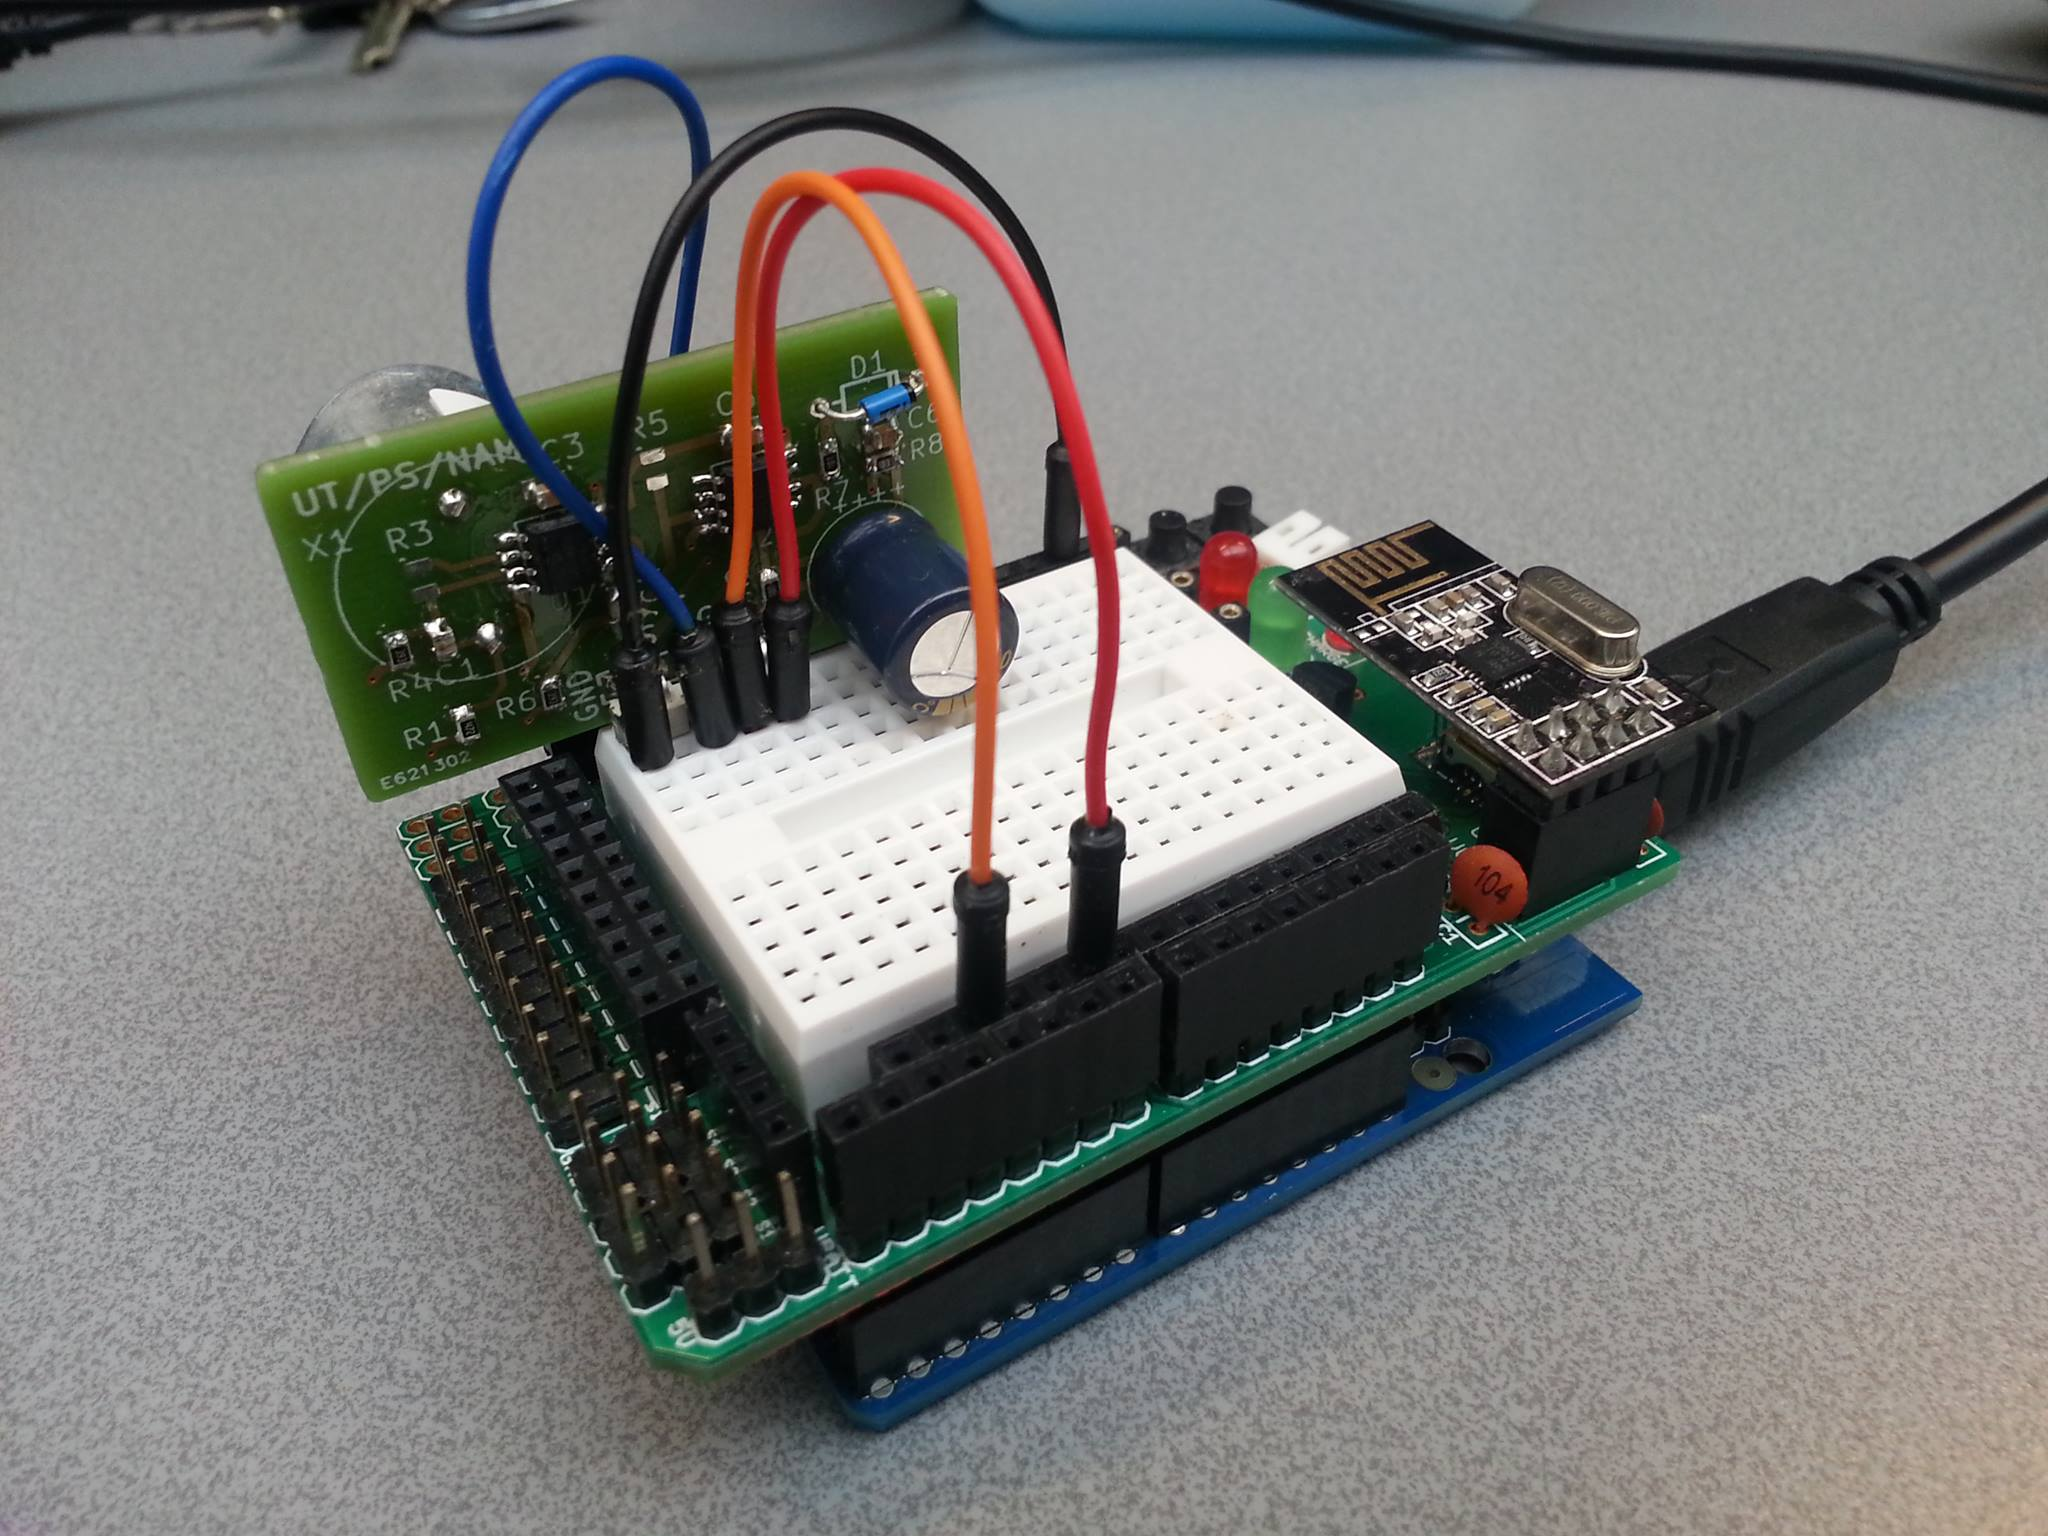
\includegraphics[scale=0.06]{achterkant.jpg}
\caption{De ontvanger (achterkant)}
\label{achterkant}
\end{figure}
\subsubsection{Zender}
Als zender is er gebruik gemaakt van vier bakens die een ultrasoon geluid uitzenden. Het signaal van deze bakens wordt verstuurd in de richting waarin ze wijzen. Deze bakens bevatten hardware die vergelijkbaar is met die van de ontvanger, met als grote verschil dat er in plaats van een ultrasoonontvanger een ultrasoonzender is gebruikt.
\\

\subsection{De software}
Om de RF24 radio aan te sturen wordt gebruik gemaakt van de opensourcesoftwarebibliotheek voor de Arduino \cite{rf24}. Met deze software kan de radio aangestuurd worden en kunnen pakketjes worden verzonden en ontvangen. De radio luistert en verstuurt pakketten over een bepaald frequentiekanaal. Het is van belang dat de radio's hetzelfde frequentiekanaal gebruiken, zodat ze met elkaar kunnen communiceren. De kanalen hebben een nummer van 0 tot en met 125. De gebruikte instellingen zijn als volgt:
\begin{itemize}
	\item Frequentiekanaal: 76 
	\item Automatisch herzenden: uit
	\item Transmissiesnelheid: 2 Mbps
	\item Adres pipe: 0xdeadbeefa1
	\item Payload-grootte: 1 byte
\end{itemize}
De ultrasoonontvanger gebruikt de volgende instellingen:
\begin{itemize}
	\item 40 kHz signaal: uit
	\item Versterking: 50x
\end{itemize}
Verder heeft de ruimte waarin de tests zijn uitgevoerd een temperatuur van $21.7\,^{\circ}{\rm C}$, wat neerkomt op een geluidssnelheid van ongeveer 344 m/s. Deze waarde is dan ook gebruikt bij de berekening van de afstand tot de bakens.\\
\\
Om de tests te kunnen uitvoeren is er gebruik gemaakt van vier bakens die met een bepaald patroon informatie verzenden. In Figuur \ref{uitzenden_bakens} is schematisch weergegeven hoe de signaalverzending werkt. In het schema zijn vier dezelfde iteraties te zien. Omdat er gebruik wordt gemaakt van vier bakens staan er vier berichten in het schema weergegeven. \\
\\
De ultrasoonontvangers waarmee de signalen van de bakens worden ontvangen werden op een afstand groter dan vijf meter zeer onnauwkeurig dus is ervoor gekozen om binnen een veld van vijf bij vijf meter te werken. In Figuur \ref{Meetopstelling} staan de vier bakens aangegeven met de oranje stippen samen met hun co\"{o}rdinaten. Met de roze stippen worden de testlocaties bedoeld waarop is getest. De bakens die zijn gebruikt versturen alleen signalen in de richting waarin ze wijzen. Hierdoor is het niet mogelijk correcte gegevens te verkrijgen wanneer er vanachter de bakens wordt gemeten. \\
\\
Tijdens het testen wordt de ontvanger op een bepaald co\"{o}rdinaat geplaatst. Het is belangrijk dat deze locatie precies is, anders ontstaat er een afwijking tussen de meetresultaten en de verwachte waarde. 
Het is van belang bij het testen dat er gebruik wordt gemaakt van een "schoon" grid. Dit houdt in, geen obstakels die de metingen zouden kunnen verstoren. Alle tests zijn "schoon"  bepaald. 
Op de volgende locaties zijn de volgende tests uitgevoerd:\\
\\
\indent Test 1: De Arduino wordt op het co\"{o}rdinaat (290, 434) geplaatst. \\
\indent Test 2: De Arduino wordt op het co\"{o}rdinaat (60, 155) geplaatst. \\
\indent Test 3: De Arduino wordt op het co\"{o}rdinaat (72, 377) geplaatst. 

\subsection{Uitgevoerde tests}
Om de afwijking van de co\"ordinaten te kunnen berekenen zijn er drie tests uitgevoerd. Deze tests zijn alle drie op exact dezelfde manier uitgevoerd, maar dan op verschillende co\"{o}rdinaten. Om ervoor te zorgen dat er een goed beeld gevormd kon worden en er voldoende resultaten zijn, is ervoor gekozen om van elke positie 26 meetresultaten te nemen en hier het gemiddelde van te nemen om het zo representatief mogelijk te maken. 

\subsection{Meetresultaten}
\label{gemiddeldes}
In Tabel \ref{table:res1}, \ref{table:res2} en \ref{table:res3} zijn de meetresultaten te zien. Er zijn  metingen verricht op drie verschillende co\"ordinaten. Voor elk co\"ordinaat is het gemiddelde van de metingen weergegeven en de afwijking ten opzichte van het co\"ordinaat waarop deze meting heeft plaatsgevonden. De volledige metingen inclusief tussenresultaten zijn te vinden in Appendix \ref{Meetresultaten}.

\begin{table}[h!]
\centering
\caption{Metingswaarden op co\"ordinaat (290, 434) in cm}\label{table:res1}
\begin{tabular}{ |l|l| }
  \hline
    gemiddelde waarde x-co\"ordinaat & gemiddelde waarde y-co\"ordinaat \\ \hline
     292,9 & 439,1 \\ \hline  \hline
  co\"ordinaat & afwijking van co\"ordinaat in cm\\ \hline 
  x & 2,9 \\ \hline
  y & 5,1 \\ \hline
  (x,y) & 5,87 \\ \hline
\end{tabular}
\end{table}

\begin{table}[h!]
\centering
\caption{Metingswaarden op co\"ordinaat (60, 155) in cm}\label{table:res2}
\begin{tabular}{ |l|l| }
  \hline
    gemiddelde waarde x-co\"ordinaat & gemiddelde waarde y-co\"ordinaat \\ \hline
     60,4 & 151,8 \\ \hline  \hline
  co\"ordinaat & afwijking van co\"ordinaat in cm\\ \hline 
  x & 0,4 \\ \hline
  y & 3,2 \\ \hline
  (x,y) & 3,22 \\ \hline
\end{tabular}
\end{table}

\begin{table}[h!]
\centering
\caption{Metingswaarden op co\"ordinaat (72,377) in cm}\label{table:res3}
\begin{tabular}{ |l|l| }
  \hline
    gemiddelde waarde x-co\"ordinaat & gemiddelde waarde y-co\"ordinaat \\ \hline
     75,6 & 379,5 \\ \hline  \hline
  co\"ordinaat & afwijking van co\"ordinaat in cm\\ \hline 
  x & 3,6 \\ \hline
  y & 2,5 \\ \hline
  (x,y) & 4,38 \\ \hline
\end{tabular}
\end{table}
\newpage
\subsection{Analyse}
Te zien is dat de metingen niet hetzelfde zijn, ze fluctueren enigszins. Een mogelijke reden hiervoor zou 
het ontvangen van echo's die weerkaatsen op objecten door de ultrasoonontvanger kunnen zijn. Deze foutieve metingen worden meegenomen in de berekening waardoor de waarde niet meer klopt. Er bleken echo's te zijn doordat er in het algoritme de afstand tot de verschillende bakens eerst wordt getoond voordat er een positie wordt berekend. Hieruit bleek dat de bakens soms elf meter van de ontvanger af stonden en dit kan alleen verklaard worden doordat er echo's zijn.\\
\\
Verder is voor het algoritme is de geluidssnelheid van belang, omdat deze \'{e}\'{e}n keer gekozen is en niet elke keer wordt aangepast aan de temperatuur en luchtvochtigheid zou deze een fluctuatie kunnen veroorzaken. Echter zijn de metingen opeenvolgend uitgevoerd en is de temperatuur niet dusdanig veranderd tijdens deze metingen dat de ingestelde geluidssnelheid de fluctuaties verschillen in waarde tussen de resultaten kan veroorzaken.

\section{Conclusie}
 De onderzoeksvraag die hier centraal staat: \textit{"Is het mogelijk om met een afwijking kleiner dan 5 procent de positie van de ontvanger in een 5 bij 5 meter veld te bepalen?"} Uit Sectie \ref{gemiddeldes} blijkt van alle drie de gemiddelde afwijkingen dat dit minder dan 25 centimeter is, nu kan geconcludeerd worden dat de afwijking minder dan 5 procent is binnen een veld van vijf bij vijf meter. Hieronder volgen een aantal aanbevelingen voor vervolgonderzoeken die uitgevoerd kunnen worden. 

\subsection{Aanbevelingen} 
 Voor een vervolgonderzoek zou er naar de volgend punten gekeken kunnen worden.
 \begin{itemize}
 	\item De arduino die tijdens dit onderzoek gebruikt is heeft veel last van bit overflow. Om de nauwkeurigheid te vergroten zou er onderzoek gedaan kunnen worden naar het gebruik van Arduino's met een grotere rekencapaciteit. Zodat op deze manier ook berekeningen gedaan kunnen worden op een afstand groter dan zes meter. 
 	\item De bakens en ontvangers die tijdens dit onderzoek gebruikt zijn zijn maar nauwkeurig tot ongeveer 5 meter. Voor een vervolg onderzoek kan er gekeken worden naar de haalbaarheid met sterkere bakens en ontvangers zodat de positiebepaling nauwkeurig blijft wanneer de afstand groter dan 5 meter bedraagt. 
 	\item Het ontworpen algoritme werkt alleen als er geen verstoringen in het veld zijn, dit wil zeggen dat er geen obstakels staan tussen het uitgezonden geluid door de bakens en de ultrasoonontvanger. Een vervolgonderzoek kan zich richten op het nauwkeurig berekenen van de positie met obstakels in het veld.  
 \end{itemize}
\newpage

%\section{References}
%\nocite{*} % Even non-cited BibTeX-Entries will be shown.
\bibliographystyle{abbrv}
\bibliography{literature}
\newpage
\appendix
\counterwithin{figure}{section}
\section{Code Trilateration}
\label{code}
    \fontsize{8pt}{8pt}\selectfont
\verbatiminput{./location/location.ino}
    \fontsize{10pt}{12pt}\selectfont
\newpage

\section{Meetresultaten}
\label{Meetresultaten}
\begin{tabular}{ |l|l| }
  \hline
  \multicolumn{2}{|c|}{(290, 434)} \\
  \hline
  x-co\"ordinaat & y-co\"ordinaat \\ \hline
     294 & 434\\ \hline
     296 & 445\\ \hline
     296 & 441\\ \hline
     293 & 434\\ \hline
     295 & 436\\ \hline
     293 & 434\\ \hline
     297 & 439\\ \hline
     294 & 432\\ \hline
     293 & 449\\ \hline
     292 & 449\\ \hline
     292 & 449\\ \hline
     293 & 449\\ \hline
     292 & 439\\ \hline
     294 & 439\\ \hline
     286 & 433\\ \hline
     286 & 433\\ \hline
     292 & 436\\ \hline
     291 & 435\\ \hline
     289 & 429\\ \hline
     295 & 436\\ \hline
     293 & 444\\ \hline
     293 & 435\\ \hline
     294 & 451\\ \hline
     293 & 433\\ \hline
     293 & 433\\ \hline
     288 & 440\\ \hline\hline
     \multicolumn{2}{|l|}{gemiddelde} \\ \hline
     292,9 & 439,1 \\ \hline
\end{tabular}
\begin{tabular}{ |l|l| }
  \hline
  \multicolumn{2}{|c|}{(60, 155)} \\
  \hline
  x-co\"ordinaat & y-co\"ordinaat \\ \hline
     59 & 137\\ \hline
     57 & 147\\ \hline
     58 & 154\\ \hline
     58 & 151\\ \hline
     60 & 157\\ \hline
     60 & 148\\ \hline
     60 & 154\\ \hline
     62 & 147\\ \hline
     63 & 151\\ \hline
     62 & 147\\ \hline
     61 & 137\\ \hline
     60 & 154\\ \hline
     60 & 150\\ \hline
     60 & 152\\ \hline
     59 & 152\\ \hline
     60 & 154\\ \hline
     61 & 151\\ \hline
     60 & 152\\ \hline
     62 & 155\\ \hline
     61 & 152\\ \hline
     61 & 155\\ \hline
     61 & 149\\ \hline
     61 & 155\\ \hline
     61 & 154\\ \hline
     60 & 152\\ \hline
     63 & 156\\ \hline\hline
     \multicolumn{2}{|l|}{gemiddelde} \\ \hline
     60,4  & 151,8 \\ \hline
\end{tabular}
\begin{tabular}{ |l|l| }
  \hline
  \multicolumn{2}{|c|}{(72, 377)} \\
  \hline
  x-co\"ordinaat & y-co\"ordinaat \\ \hline
     75 & 378\\ \hline
     77 & 383\\ \hline
     76 & 382\\ \hline
     76 & 381\\ \hline
     75 & 378\\ \hline
     74 & 374\\ \hline
     74 & 377\\ \hline
     75 & 378\\ \hline
     76 & 382\\ \hline
     77 & 387\\ \hline
     76 & 388\\ \hline
     78 & 382\\ \hline
     74 & 387\\ \hline
     76 & 378\\ \hline
     74 & 382\\ \hline
     76 & 381\\ \hline
     77 & 377\\ \hline
     75 & 382\\ \hline
     77 & 377\\ \hline
     75 & 380\\ \hline
     76 & 374\\ \hline
     73 & 382\\ \hline
     75 & 377\\ \hline
     74 & 376\\ \hline
     77 & 378\\ \hline
     78 & 380\\ \hline\hline
     \multicolumn{2}{|l|}{gemiddelde} \\ \hline
     75,6 & 379,5 \\ \hline 
\end{tabular}
\newline
\begin{tabular}{ |l|p{3,1cm}| }
  \hline
  \multicolumn{2}{|c|}{afwijking(290, 434) in cm} \\
  \hline
  x & 2,9 \\ \hline
  y & 5,1 \\ \hline
  (x,y) & 5,87 \\ \hline
\end{tabular}
\begin{tabular}{ |l|p{3,1cm}| }
  \hline
  \multicolumn{2}{|c|}{afwijking (60, 155) in cm} \\
  \hline
  x & 0,4 \\ \hline
  y & 3,2 \\ \hline
  (x,y) & 3,22 \\ \hline
\end{tabular}
\begin{tabular}{ |l|p{3,1cm}| }
  \hline
  \multicolumn{2}{|c|}{afwijking(72,377) in cm} \\
  \hline
  x & 3,6 \\ \hline
  y & 2,5 \\ \hline
  (x,y) & 4,38 \\ \hline
\end{tabular}

\end{document}